\iffalse
\let\negmedspace\undefined
\let\negthickspace\undefined
\documentclass[a4,12pt,onecolumn]{IEEEtran}
\usepackage{amsmath,amssymb,amsfonts,amsthm}
\usepackage{algorithmic}
\usepackage{graphicx}
\usepackage{textcomp}
\usepackage{xcolor}
\usepackage{txfonts}
\usepackage{listings}
\usepackage{enumitem}
\usepackage{mathtools}
\usepackage{gensymb}
\usepackage[breaklinks=true]{hyperref}
\usepackage{tkz-euclide}
\usepackage{listings}
\usepackage{circuitikz}
\usepackage{gvv}
\begin{document}
\title{Discrete Assignment}
\author{Shravya Kantayapalam\\ EE23BTECH11030}
\maketitle

\begin{enumerate}
    \item \textbf{Question 11.9.4.9}:
    Find the sum to $n$ terms of the series whose $n$th term is given by $n^2 + 2^n$?
 \end{enumerate}  
    \textbf{Solution}:
\fi 

\begin{table}[htbp]
    \centering
    \caption{Input Parameters}
    \begin{tabular}{|l|l|l|}
    \hline
    \textbf{Variable} & \textbf{Description} & \textbf{Value} \\
    \hline
    \( x(n) \) & \( n \)-th term of sequence & \( (n^2 + 2^n)u(n) \) \\
    \hline
    \end{tabular}
\end{table}
\begin{align}
x(n)&=(n^2+2^n)u(n)\\
2^n \cdot u(n) &\xleftrightarrow{\text{Z}} \frac{1}{1 - 2z^{-1}} \\
n^2u(n) &\xleftrightarrow{\mathcal{Z}} \frac{z^{-1}(1+z^{-1})}{(1-z^{-1})^3} \quad \abs{z}>1 \\ 
\text{Taking } z \text{ transform :}\\
X(z)&=\frac{z^{-1}(z^{-1} + 1)}{(1 - z^{-1})^3} +\frac{1}{1 - 2z^{-1}}\\
Y(z)&=X(z)U(z)\\
Y(z)&=\brak{\frac{z^{-1}(z^{-1} + 1)}{(1 - z^{-1})^3} +\frac{1}{1 - 2z^{-1}}}\brak{\frac{1}{1-z^{-1}}}\\
Y(z)&=\frac{z^{-1}(1+z^{-1})}{(1-z^{-1})^4}+\frac{2}{1-2z^{-1}}-\frac{1}{1-z^{-1}}\\
\text{Taking inverse } \mathcal{Z} \text{ transform :}\\
y(n)&=\frac{n^2(n^2-1)}{3}u(n)+2.2^nu(n)-u(n)\\
y(n)&=\brak{\frac{n^2(n^2-1)}{3}+2^{n+1}-1}u(n)
\end{align}
\begin{figure}[ht]
    \centering
    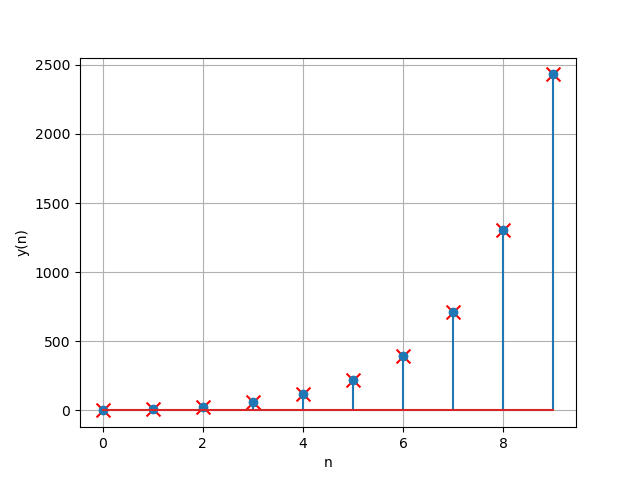
\includegraphics[width=\columnwidth]{figs/main.png}
    \caption{Graph of $y(n)$ }
\end{figure}


